\documentclass[20pt,margin=1in,innermargin=-4.5in,blockverticalspace=-0.25in]{tikzposter}
\geometry{paperwidth=42in,paperheight=30in}
\usepackage[utf8]{inputenc}
\usepackage{csquotes}
% \usepackage[estonian]{babel}
\usepackage{amsmath}
\usepackage{amsfonts}
\usepackage{amsthm}
\usepackage{amssymb}
\usepackage{mathrsfs}
\usepackage{graphicx}
\usepackage{adjustbox}
\usepackage{enumitem}
\usepackage{xcolor}
\usepackage{./unitartu-theme}
\usepackage{mwe} % for placeholder images
\usepackage{anyfontsize}

\graphicspath{{../../apps/aco_tsp/test/results/}}
% set theme parameters
\tikzposterlatexaffectionproofoff
\usetheme{UniTartuTheme}
\usecolorstyle{UniTartuStyle}

\usepackage[scaled]{helvet}
\renewcommand\familydefault{\sfdefault} 
\renewcommand{\vec}[1]{\bm{#1}}
\newcommand{\Tr}{\text{Tr}}
\usepackage[T1]{fontenc}
\usepackage{multicol}

\title{Distributed Ant Colony Optimization on the Travelling Salesman Problem}
\author{\textbf{Andrea Malleo}
}
\institute{Distributed Systems Fall 2021\\
            %\textsuperscript{2}Institute of Mathematics, University of Tartu % Add 2nd author institute
            }
%\titlegraphic{\includegraphics[width=0.20\linewidth]{unitartu_compact.png}}

% begin document
\begin{document}
\maketitle
\centering
\begin{columns}
    \column{0.25}
    \block{Problem}{
        \begin{itemize}
        {\LARGE
            \item ACO is a probabilistic technique that leverages a distributed system of independent software agents 
                to search the solution space. 
            
        \item Effort has been made to speed up the execution by parallelizing independent runs of the sequential algorithm
        \item Less work has been concentrated on implementing a single ant colony
         as a distributed system.
        \item Elixir uses the actor model, which achieves concurrency via independent computing processes that
        communicate via asynchronous message passing instead of any shared memory.

        \item What levels of speedup can we see over the serialized method as we dial up the number 
              of ants in the simulated colony?
        }
    \end{itemize}
    }
    \block{Results}{
        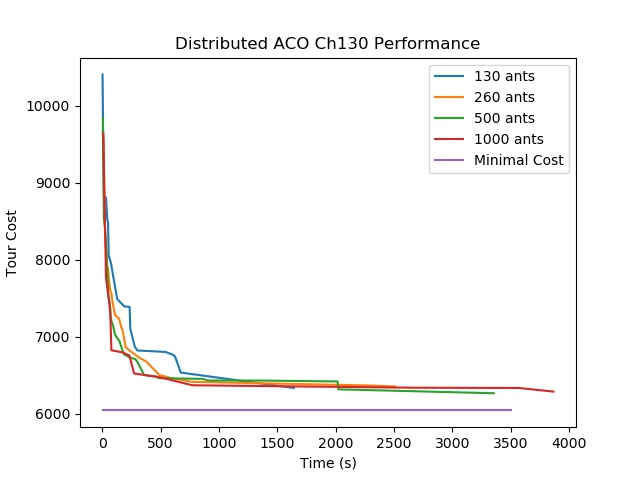
\includegraphics[width=1.0\linewidth,height=15.0cm]{ch130_performance_vs_ants.jpg}
       }

    \block{Process Architecture}{
        \begin{multicols*}{2}
            \begin{enumerate}
                \item  Ant
                \item  Graph manager 
                \item Pheromone manager
                \item Ant manager
                \item Colony manager
           \end{enumerate}
        \end{multicols*}
    }
   

    \column{0.50}
    \block{Main Idea}{
        \begin{center}

        \fontsize{100pt}{120pt}\selectfont A Distributed Implementation of Ant Colony Optimization

        \vspace{10mm}
        Using the Actor Model of Concurrency \\

        \vspace{10mm}

        Provides a clear, correct method of solving the TSP \\

        \vspace{10mm}

        With Speed Benefits over a Serialized 
        Implementation that increase with problem scale.

        \end{center}
    }

    \column{0.25}
    \block{Methods}{
        \begin{itemize}
        {\LARGE
            \item Naturally, the ACO algorithm is iterative. Each round, every ant individually completes
        a tour of the graph. The paths are mostly random at first, favoring small steps, and
        incorporating  over time the collective intelligence of the colony of ants
        by weighting paths more heavily if they produced shorter tours on previous rounds by 
        other ants. 
        
        \item The goal is for the positive feedback mechanism, encapsulated in the pheremone matrix,
        to lead to convergence to the best path.

        \item The Actor model for synchronization greatly simplifies the shared read 
        and write access of the pheremone matrix among all of the 'ants' by collecting and sharing 
        path costs and pheremone values via messages. 
        }
        \end{itemize}

    }
    \block{Results}{
       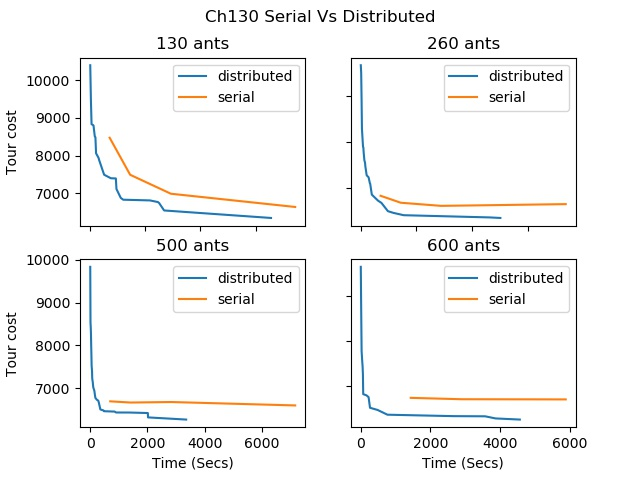
\includegraphics[width=1.0\linewidth,height=20.0cm]{ch130_serial_vs_dist.jpg}
       }

    

    
 
\end{columns}
\end{document}